% manuscript.tex — journal-neutral draft (article class). Compile: latexmk -pdf manuscript.tex
% Every number in this file is taken from a repository file named in figures_and_tables_plan.md.
% Claims that the current evidence does not support are marked \evreq{...}.
\documentclass[11pt]{article}
\usepackage[utf8]{inputenc}
\usepackage[T1]{fontenc}
\usepackage{lmodern}
\usepackage[margin=2.5cm]{geometry}
\usepackage{amsmath,amssymb,amsthm}
\usepackage{graphicx}
\usepackage{booktabs}
\usepackage{tabularx}
\usepackage{xcolor}
\usepackage[numbers,sort&compress]{natbib}
\usepackage[hidelinks]{hyperref}
\usepackage{microtype}

\graphicspath{{figures/}{../docs/figures/}}
\newcommand{\evreq}[1]{\textcolor{red!70!black}{\textbf{[EVIDENCE REQUIRED:} #1\textbf{]}}}
\newtheorem{proposition}{Proposition}
\newtheorem{lemma}{Lemma}
\newtheorem{corollary}{Corollary}
\theoremstyle{definition}
\newtheorem{definition}{Definition}
\newtheorem{remark}{Remark}
\theoremstyle{remark}
\newtheorem{hypothesis}{Hypothesis}

\title{Filter-Induced and Learned Deadlocks in Safety-Filtered Reinforcement Learning for Mobile Robot Navigation}
\author{Pouya Bathaei Pourmand}
\date{Draft, \today}

\begin{document}
\maketitle

\begin{abstract}
A control-barrier-function (CBF) safety filter can make a learned navigation policy collision-free, but the robot may then stall in front of an obstacle and time out. We analyse such deadlocks for a unicycle robot whose speed is limited by a one-step discrete-time CBF filter. Two elementary properties of the filter frame the analysis. Because the next position depends only on the speed, the one-step safety guarantee does not depend on the commanded turn rate, so any modification of the turn rate preserves it. Near the keep-out boundary, the set of headings that permit motion shrinks to the half-plane that points away from the obstacle. We then classify the timeouts of ten proximal-policy-optimisation (PPO) agents and two classical controllers on 300 seeded test scenarios. In every scenario, a geometric oracle confirms that a path keeping the safety margin exists. Two mechanisms dominate, and they depend on how the agent was trained. Agents trained without the filter and run with it are \emph{blocked by the filter} at the boundary (141 of 175 expert timeouts). Agents trained with the filter mostly \emph{stop by themselves} before the boundary (122 of 195), so the filter is not the immediate cause. In paired comparisons on the expert stage, training with the filter lowered the filter-blocked rate by 14.8 percentage points (95\,\% interval [5.6, 24.4]) and raised the self-stop rate by 17.6 points [8.2, 27.0]. Sampling actions instead of using the policy mean removed most self-stops but no filter-blocked stalls. Both training contrasts replicated in a pre-registered evaluation on 500 previously unused scenarios. In the same evaluation, a test-time heading modification that cannot weaken the safety guarantee lowered the filter-blocked rate of agents trained without the filter by 7.4 points [4.8, 10.2] and raised their success by 7.2 points [5.0, 9.7], with zero collisions. It left self-stops unchanged. Self-stops did not disappear with longer training: they were more frequent at the final training checkpoints than at the selected ones. All results are from simulation with exact state and static circular obstacles, and they do not establish real-world safety. \evreq{Results of the correction-penalty baseline (E1) must be added before submission; see minimum\_experiments.md.}
\end{abstract}

\noindent\textbf{Keywords:} safe reinforcement learning; control barrier functions; safety filter; deadlock; mobile robot navigation; liveness.

%=====================================================================
\section{Introduction}
%=====================================================================
Safety filters are a common way to make learned controllers usable in safety-critical settings~\cite{hsu2024safetyfilter,brunke2022safe}. The learned policy proposes an action, and a filter, often a control barrier function (CBF) quadratic program~\cite{ames2017cbfqp,ames2019cbf}, replaces it with the closest action that keeps the system in a safe set. In robot navigation, the safe set excludes a margin around every obstacle, and the filter guarantees under its modelling assumptions that the robot never enters that margin.

The guarantee says nothing about reaching the goal. For model-based nominal controllers it is known that CBF filters can create undesired stable equilibria on the boundary of the safe set~\cite{reis2021undesired,tan2024undesired}, and multi-robot CBF controllers can deadlock~\cite{grover2023deadlock,jankovic2024liveness,chandra2025deadlock}. When the nominal controller is a reinforcement-learning (RL) policy, the situation is less clear. The policy may have been trained with the filter in the loop~\cite{pizarro2025filtering,yang2026cbfrl,krasowski2023provably}, it reacts to observations rather than to the true state, and its behaviour near obstacles is learned rather than designed. Recent work shows that RL under a perfect, least-restrictive filter loses no optimality~\cite{oh2026optimal}, and that adding a penalty on the filter's correction improves the performance of filter-trained agents in trajectory tracking~\cite{pizarro2025filtering}.

That safety mechanisms can impede task progress has been observed before. Yang et al.\ note that a policy unaware of the CBF can behave conservatively~\cite{yang2026cbfrl}. Thumm et al.\ note that fail-safe interventions can cause abrupt braking or aggressive steering~\cite{thumm2023reducing}. Banerjee et al.\ note that shields with fixed backup policies often hinder task progress~\cite{banerjee2024dmps}. In crowd navigation, a planner may decide that all forward paths are unsafe and freeze the robot, although a feasible path typically exists~\cite{trautman2010unfreezing}. Our targeted search did not find a study that, for a single robot driven by a learned policy behind a CBF filter, (i)~separates stalls caused by the filter from stops commanded by the policy, (ii)~checks every failure against a geometric feasibility oracle, and (iii)~relates the dominant mechanism to how the policy was trained. This is the gap we address. The search was targeted, not systematic, so the claim is limited to the work we examined.

This paper studies that question in a deliberately simple and fully reproducible setting. The robot is a unicycle, the obstacles are static circles, and the filter is a one-step discrete-time CBF on the speed~\cite{agrawal2017discrete}. The setting is simple enough that the filter's behaviour can be analysed exactly, and that every timeout can be checked against a geometric feasibility oracle.

\paragraph{Research questions.}
\begin{itemize}
  \item[RQ1] Which properties of a one-step discrete-time CBF speed filter determine where and how a filtered robot can stall?
  \item[RQ2] By which mechanisms do learned policies deadlock behind such a filter, and does training with the filter change the mechanism?
  \item[RQ3] Which simple remedies (stochastic deployment, the published correction penalty, heading-level modification) remove which mechanism? \evreq{Stochastic deployment and a test-time heading modification have been evaluated; the correction penalty (E1) has not.}
\end{itemize}

\paragraph{Contributions.}
\begin{enumerate}
  \item Elementary properties of the one-step speed filter for the unicycle (Section~\ref{sec:theory}). They follow directly from the forward-Euler model and are not new theory. We state them because they determine which remedies can work and give testable predictions. One-step safety is independent of the commanded turn rate (Lemma~\ref{prop:heading}), so heading-level remedies keep the guarantee. The set of headings that permit motion collapses as the barrier approaches zero (Proposition~\ref{prop:cone}), which gives a stall bound (Corollary~\ref{cor:stall}). At steps where the policy commands a near-zero speed, no test-time speed limit can make the robot move (Lemma~\ref{prop:typeII}). This says nothing about earlier steps or about training.
  \item A diagnostic procedure for deadlocks in this filtered navigation setting. It combines a geometric feasibility oracle, a stall taxonomy (filter-blocked vs.\ self-stop) and uncertainty estimates over both training seeds and test scenarios (Section~\ref{sec:setup}). The oracle and the class thresholds are specific to static circular obstacles and a unicycle, but the procedure can be adapted to other settings.
  \item Empirical evidence from ten PPO agents and two classical controllers (Section~\ref{sec:results}). The two stall mechanisms exist, and they depend on the training setup. They respond differently to stochastic deployment and to a heading modification. They replicate on previously unused scenarios. The filter-blocked stalls match the geometry predicted by Proposition~\ref{prop:cone}, and self-stops are not an artefact of early checkpoint selection.
\end{enumerate}
We do not claim a new safety filter or a new training algorithm. The safety proof of the filter is standard~\cite{agrawal2017discrete} and is restated only for completeness. The correction penalty is the established method of Pizarro Bejarano et al.~\cite{pizarro2025filtering}, and similar penalties on blocked or corrected actions appear in earlier work~\cite{alshiekh2018shielding,saunders2018trial,krasowski2023provably}. We implement only its correction-penalty term, $\alpha\lVert u-u^{\mathrm{exec}}\rVert^2$ with $\alpha=1$. Here $u$ is the policy's sample and $u^{\mathrm{exec}}$ is the executed action after the action bounds and our one-step filter. Our filter replaces their predictive safety filter, and we do not use their safe resets. We use this term as a baseline. What is new is the question it is used to answer: does it remove either stall mechanism in navigation, and which one (RQ3)?

%=====================================================================
\section{Related work}
%=====================================================================
\paragraph{Safety filters and CBFs.} CBF quadratic programs~\cite{ames2017cbfqp,ames2019cbf} and their discrete-time form~\cite{agrawal2017discrete,zeng2021mpcdcbf} are the standard tools for enforcing state constraints around arbitrary nominal controllers. High-order CBFs handle constraints with higher relative degree~\cite{xiao2022hocbf}. Predictive and reachability-based filters offer less conservative alternatives at higher computational cost~\cite{wabersich2021psf,hsu2024safetyfilter}. Robust, measurement-robust and stochastic variants address model and state uncertainty~\cite{kolathaya2019issf,cosner2021mrcbf,cosner2023stochastic,das2026robust}.

\paragraph{Undesired equilibria and deadlock.} Reis et al.~\cite{reis2021undesired} showed that CBF-QPs can introduce asymptotically stable equilibria on the safe-set boundary, and Tan and Dimarogonas~\cite{tan2024undesired} characterised them in general. In multi-robot navigation, deadlock was analysed as a force equilibrium on the boundary~\cite{grover2021deadlock,grover2023deadlock} and resolved through instability of the deadlock set~\cite{jankovic2024liveness} or with discrete-time CBFs~\cite{chandra2025deadlock}. All of these analyses assume a model-based nominal controller. Potential fields have the analogous problem of local minima~\cite{koren1991potential}. In crowd navigation, the ``freezing robot problem'' describes a planner that decides all forward paths are unsafe, so that the robot freezes, although a feasible path typically exists~\cite{trautman2010unfreezing}. The self-stops in Section~\ref{sec:results} resemble this behaviour, but they come from a learned policy behind a filter, not from a planner. Reach-avoid RL gives safety and liveness guarantees by learning a reach-avoid value function~\cite{hsu2021reachavoid}, a different design from post-hoc filtering.

\paragraph{Safety filters and shields in RL.} Shields replace unsafe actions during learning~\cite{alshiekh2018shielding,carr2023shielding}, and CBF filters have been combined with RL in several ways~\cite{cheng2019endtoend,emam2025robust,xiao2023barriernet,pham2018optlayer}. Krasowski et al.~\cite{krasowski2023provably} compare action replacement, projection and masking, and report that a penalty on interventions helps. Thumm et al.~\cite{thumm2023reducing} modify the agent's action proactively to reduce fail-safe interventions, which can otherwise cause abrupt braking or aggressive steering. Banerjee et al.~\cite{banerjee2024dmps} replace the fixed backup policy of model predictive shielding, which they note often hinders task progress, with a local planner that selects recovery actions using the learned policy's value estimates. Pizarro Bejarano et al.~\cite{pizarro2025filtering} study filtering during training, a correction penalty and safe resets for PPO on quadrotor trajectory tracking; they report chattering, but their task has no obstacles and they do not analyse stalls. Yang et al.~\cite{yang2026cbfrl} filter rollouts and add a CBF reward term so that the policy can be deployed without a filter. The term penalises violations of the CBF condition by the policy's action, and the distance between the policy's action and the filtered action. Their navigation agent is a single integrator, which has no heading, so the heading geometry of Section~\ref{sec:theory} does not arise. They report success rates, but they do not analyse timeouts or stalls. Oh et al.~\cite{oh2026optimal} prove that RL under a perfect, least-restrictive filter, one that intervenes only when the nominal action would leave the maximal controlled-invariant set, preserves optimality. CBF-based safe RL for navigation includes~\cite{song2022lidar,marzari2025probabilistic,xie2025certificated,guo2025radar}. Barriers synthesised online from range data remove the known-map assumption~\cite{keyumarsi2024lidar,long2021barrier}.

\paragraph{Policy gradients under clipped or projected actions.} When an action is clipped or projected before execution, many sampled actions lead to the same executed action, and therefore to the same return. Fujita and Maeda~\cite{fujita2018capg} study clipping to action bounds. They propose an estimator that uses the clipping and prove that it is unbiased and has lower variance than the conventional estimator, which ignores the bounds. Chou et al.~\cite{chou2017beta} argue that bounded actions bias the gradient of a Gaussian policy, and propose a Beta policy. In action-constrained RL, projection-based methods can suffer from a zero-gradient problem caused by the coupling between the policy gradient and the projection~\cite{lin2021zerogradient}. Gros et al.~\cite{gros2020projection} find projection onto a safe set generally disruptive for Q-learning, and give corrections that keep policy gradients unbiased. None of these works studies navigation stalls. We use them to frame, not to establish, a hypothesis about self-stops (Section~\ref{sec:discussion}).

\paragraph{Evaluation practice.} RL results vary strongly between seeds~\cite{henderson2018matters}, and few-run studies need interval estimates rather than point estimates~\cite{agarwal2021precipice}. Navigation benchmarks such as BARN~\cite{perille2020barn} and Arena-Rosnav~\cite{kastner2023arena}, and community guidelines~\cite{francis2025principles}, stress classical baselines and standardised metrics.

Table~\ref{tab:related} positions this work. Entries for other papers reflect the parts we read (see LITERATURE\_REVIEW.md and literature\_review\_gap\_analysis.md for the reading depth); ``n.r.'' means not reported in those parts, not that the paper lacks the property.

\begin{table}[t]
\centering\small
\caption{Positioning. Y = yes; -- = no; n.r. = not reported in the parts read; (Y) = partly.}
\label{tab:related}
\begin{tabularx}{\linewidth}{@{}Xcccccc@{}}
\toprule
Work & Learned & Filter in & Navigation & Deadlock / & Equilibria of & Feasibility \\
 & policy & training & & liveness & learned policy & oracle \\
\midrule
Reis et al.~\cite{reis2021undesired}; Tan \& Dimarogonas~\cite{tan2024undesired} & -- & -- & (Y) & Y & -- & -- \\
Grover et al.~\cite{grover2023deadlock}; Jankovic et al.~\cite{jankovic2024liveness}; Chandra et al.~\cite{chandra2025deadlock} & -- & -- & Y & Y & -- & n.r. \\
Krasowski et al.~\cite{krasowski2023provably} & Y & Y & -- & n.r. & -- & -- \\
Thumm et al.~\cite{thumm2023reducing} & Y & Y & (Y) & n.r. & -- & n.r. \\
Pizarro Bejarano et al.~\cite{pizarro2025filtering} & Y & Y & -- & chattering & -- & -- \\
Oh et al.~\cite{oh2026optimal} & Y & Y & n.r. & n.r. & -- & -- \\
Yang et al.~\cite{yang2026cbfrl} & Y & Y & (Y)$^{a}$ & -- & -- & -- \\
Banerjee et al.~\cite{banerjee2024dmps} & Y & Y & n.r. & (Y)$^{b}$ & n.r. & n.r. \\
Marzari et al.~\cite{marzari2025probabilistic}; Guo et al.~\cite{guo2025radar} & Y & (Y) & Y & -- & -- & -- \\
\textbf{This work} & Y & Y & Y & Y & Y & Y \\
\bottomrule
\end{tabularx}
\par\smallskip\raggedright\footnotesize $^{a}$\,Navigation with a single integrator, which has no heading; success rates reported, timeouts not analysed. $^{b}$\,Notes that backup-policy shields often hinder task progress; navigation not stated in the abstract.
\end{table}

%=====================================================================
\section{Problem formulation}\label{sec:problem}
%=====================================================================
\paragraph{Robot and environment.} The robot state is $x_t=(p_t,\theta_t)$ with position $p_t\in[0,W]^2$, $W=10$\,m, and heading $\theta_t$. The command is $u_t=(v_t,\omega_t)\in\mathcal U=[0,v_{\max}]\times[-\omega_{\max},\omega_{\max}]$ with $v_{\max}=1$\,m/s and $\omega_{\max}=1$\,rad/s. The simulator integrates
\begin{equation}\label{eq:dyn}
  p_{t+1}=p_t+v_t\,\Delta t\, e(\theta_t),\qquad \theta_{t+1}=\theta_t+\omega_t\Delta t,\qquad e(\theta)=(\cos\theta,\sin\theta)^\top,
\end{equation}
with $\Delta t=0.1$\,s. Obstacles are static discs with centres $c_i$ and radii $R_i\in[0.3,0.8]$\,m; the robot is a disc of radius $r=0.3$\,m.

\paragraph{Barriers and filter.} For a safety margin $d$ (0.3\,m) and a wall margin $m$ (0.1\,m), define
\begin{equation}\label{eq:barrier}
\begin{aligned}
  h_i(p)&=\lVert p-c_i\rVert-(R_i+r+d) &&\text{(obstacle $i$)},\\
  h_{W}(p)&\in\{p_x-(r+m),\;W-p_x-(r+m),\;p_y-(r+m),\;W-p_y-(r+m)\} &&\text{(walls)}.
\end{aligned}
\end{equation}
The safe set is $\mathcal S=\{p: h_k(p)\ge 0\ \forall k\}$. The closing rate per unit speed is $a_i(p,\theta)=e(\theta)^\top(c_i-p)/\lVert c_i-p\rVert$ for an obstacle, and $-\cos\theta,\cos\theta,-\sin\theta,\sin\theta$ for the four walls. With $\gamma=0.5\,\mathrm{s}^{-1}$ (so $\gamma\Delta t=0.05\le 1$), the filter returns
\begin{equation}\label{eq:filter}
  F(x,u)=\big(\min\{\operatorname{clip}(v),\bar v(x)\},\ \operatorname{clip}(\omega)\big),\qquad
  \bar v(x)=\min\Big\{v_{\max},\ \min_{k:\,a_k>0}\frac{\gamma\,h_k(p)}{a_k(p,\theta)}\Big\}.
\end{equation}
Because every constraint bounds the single variable $v$, \eqref{eq:filter} is the exact solution of $\min_{v}(v-v^{\mathrm{nom}})^2$ subject to $a_k v\le\gamma h_k$ and $0\le v\le v_{\max}$.

\paragraph{Policies.} A policy maps an observation $o_t$ to a nominal command. The observation contains the noisy normalised position, $\sin\theta$ and $\cos\theta$, goal distance and bearing, a proximity feature, and 16 range readings up to 3\,m. The closed loop is $x_{t+1}=f(x_t,F(x_t,\pi(o_t)))$. An episode succeeds when the goal is within 0.5\,m; it ends with a collision if the robot body touches an obstacle or leaves the workspace; otherwise it times out after 200/300/400 steps (beginner/intermediate/expert).

\begin{definition}[Stall classes]\label{def:stall}
A timeout is a \emph{stall} if the net displacement over its last $K=100$ steps is below $\delta=0.10$\,m. A stall is
(i) \emph{filter-blocked} (Type~I) if the filter reduced the commanded speed in at least half of those steps;
(ii) a \emph{self-stop} (Type~II) if, in at least half of them, the policy itself commanded a speed of at most $10^{-3}$\,m/s;
(iii) \emph{other} otherwise. A timeout that is not a stall is \emph{moving}.
\end{definition}

%=====================================================================
\section{Analysis of the one-step speed filter}\label{sec:theory}
%=====================================================================
The statements in this section follow directly from the model \eqref{eq:dyn}--\eqref{eq:filter}, and none of them requires new theory. We state them because they rule out some remedies and give the predictions that Section~\ref{sec:results} tests.

\begin{lemma}[Forward invariance~\cite{agrawal2017discrete}]\label{lem:inv}
If $p_0\in\mathcal S$ and $u_t=F(x_t,\cdot)$ for all $t$, then $h_k(p_{t+1})\ge(1-\gamma\Delta t)h_k(p_t)$ for every barrier $k$. In particular, $h_k(p_t)>0$ for all $t$ if $h_k(p_0)>0$.
\end{lemma}
\begin{proof}
By convexity of the norm, $\lVert p_{t+1}-c_i\rVert\ge\lVert p_t-c_i\rVert-\Delta t\,v_t\,a_i(p_t,\theta_t)$. If $a_i>0$, the filter enforces $v_t a_i\le\gamma h_i(p_t)$; if $a_i\le 0$, the barrier cannot decrease. Wall barriers are affine in $p$, so the same bound holds with equality. Strict positivity follows from $\gamma\Delta t<1$.
\end{proof}

\begin{lemma}[Turn-rate independence]\label{prop:heading}
Let $\psi:\mathcal X\times\mathcal U\to[-\omega_{\max},\omega_{\max}]$ be any map, and let $F_\psi(x,u)=(\min\{\operatorname{clip}(v),\bar v(x)\},\psi(x,u))$. Then Lemma~\ref{lem:inv} holds for $F_\psi$.
\end{lemma}
\begin{proof}
By \eqref{eq:dyn}, $p_{t+1}$ depends only on $(p_t,\theta_t,v_t)$, and $\bar v(x_t)$ depends only on $(p_t,\theta_t)$. The turn rate $\omega_t$ affects only $\theta_{t+1}$, which the filter evaluates again at step $t+1$. The proof of Lemma~\ref{lem:inv} therefore applies at every step, whatever $\psi$ returns.
\end{proof}

\begin{remark}
Lemma~\ref{prop:heading} is the discrete-time counterpart of a known structural fact. In continuous time, the position barrier has relative degree two with respect to $\omega$, which is the situation high-order CBFs address~\cite{xiao2022hocbf}. It has two practical consequences here. First, the one-step filter can never \emph{steer} the robot away from an obstacle: only the policy, or a heading modification $\psi$, can do so. Second, heading-level remedies for deadlock, such as a tangential turn when the speed limit is active, inherit the safety guarantee without further proof.
\end{remark}

\begin{proposition}[Collapse of the admissible headings]\label{prop:cone}
Fix $p$ with $0\le h_i(p)\le\varepsilon$ for an obstacle $i$, and a speed $\underline v>0$. Every heading $\theta$ with $\bar v(p,\theta)\ge\underline v$ satisfies $a_i(p,\theta)\le\gamma\varepsilon/\underline v$; that is, the angle between $e(\theta)$ and the direction to $c_i$ is at least $\arccos(\min\{1,\gamma\varepsilon/\underline v\})$. As $\varepsilon\to0$, this set of headings approaches the closed half-circle $\{\theta: a_i(p,\theta)\le0\}$.
\end{proposition}
\begin{proof}
If $a_i(p,\theta)>0$, then $\bar v\le\gamma h_i/a_i\le\gamma\varepsilon/a_i$, and $\bar v\ge\underline v$ requires $a_i\le\gamma\varepsilon/\underline v$. If $a_i\le0$, the inequality holds trivially.
\end{proof}

\begin{corollary}[Stall bound]\label{cor:stall}
If, over $K$ consecutive steps, $h_i(p_t)\le\varepsilon$ and $a_i(p_t,\theta_t)\ge\bar a>0$, then the robot moves at most $K\Delta t\,\gamma\varepsilon/\bar a$, whatever speed the policy commands. For a head-on approach ($a_i\equiv1$) at the speed limit, $h_i(p_{t+1})=(1-\gamma\Delta t)\,h_i(p_t)$ holds with equality, so the barrier decays geometrically and the robot approaches, but never reaches, the boundary.
\end{corollary}
\begin{proof}
The displacement per step is $v_t\Delta t\le\bar v\Delta t\le\gamma\varepsilon\Delta t/\bar a$. For straight motion toward the centre, the convexity bound in Lemma~\ref{lem:inv} is tight, giving the stated equality.
\end{proof}

\begin{lemma}[Test-time speed limits at near-zero speed commands]\label{prop:typeII}
Let $F'$ be any filter whose executed speed satisfies $0\le v^{\mathrm{exec}}\le\operatorname{clip}(v^{\mathrm{nom}})$, and let $\underline v\ge0$. At every step where the deterministic policy commands $\pi_v(o)\le\underline v$, the executed speed under $F'$ is at most $\underline v$, as it is without a filter; if $\pi_v(o)\le0$, it is exactly $0$. In particular, at the steps of Definition~\ref{def:stall} where the policy commands at most $\underline v=10^{-3}$\,m/s, no test-time speed limit can make the robot move faster than it would without a filter. At these steps, only a different command from the policy can produce motion.
\end{lemma}
\begin{proof}
$0\le v^{\mathrm{exec}}\le\operatorname{clip}(\pi_v(o))\le\max\{0,\underline v\}=\underline v$, and $\operatorname{clip}(\pi_v(o))=0$ if $\pi_v(o)\le0$.
\end{proof}
Lemma~\ref{prop:typeII} concerns only the steps at which the policy commands a near-zero speed. It says nothing about:
\begin{itemize}
  \item the other steps of a stall, at which the policy may command a larger speed;
  \item how a different speed limit at earlier steps would change the trajectory, and with it the later observations;
  \item the effect of the filter during training.
\end{itemize}

Proposition~\ref{prop:cone} and Lemma~\ref{prop:typeII} give testable predictions. Filter-blocked stalls should occur at $h\approx0$ with headings within $90^\circ$ of the obstacle direction. Self-stops should occur at $h>0$. At their stopping steps, the speed should be set by the policy's command, not by the test-time speed limit.

%=====================================================================
\section{Experimental setup}\label{sec:setup}
%=====================================================================
\paragraph{Agents.} PPO~\cite{schulman2017ppo} with separate $256\times256$ tanh actor and critic networks, a diagonal Gaussian policy whose samples are clipped by the environment, generalised advantage estimation and bootstrapping at time-limit truncations. Training ran for $10^6$ steps over a three-stage curriculum (beginner, intermediate, expert; advance at 70\,\% rolling success). Five seeds (0--4) were trained without the filter and five with the filter in the loop. In the filtered runs, the buffer stores the policy's own sample, as in~\cite{pizarro2025filtering}. The checkpoint with the highest success on 60 validation episodes (20 per stage), on seeds disjoint from the test seeds, was kept. One hyperparameter set was used for both variants and was not tuned for the filtered setting. All ten runs reached the expert stage within 43k--76k steps.

\paragraph{Baselines.} A go-to-goal heading controller, which ignores obstacles, and a hand-tuned artificial potential field on the range readings~\cite{koren1991potential}. \evreq{Published baselines are missing: correction-penalty PPO~\cite{pizarro2025filtering} (E1), PPO-Lagrangian~\cite{stooke2020pid}, and a classical local planner such as DWA~\cite{fox1997dwa} or MPC with a DT-CBF~\cite{zeng2021mpcdcbf}.}

\paragraph{Test scenarios.} 100 seeded scenarios per stage (seed bases $2\cdot10^6+10^5 s$). The expert stage has 8--12 obstacles. A grid oracle (5\,cm, 8-connected Dijkstra on the free space inflated by $r+d$) found a margin-keeping path in all 300 scenarios. Two properties of the generator must be kept in mind:
\begin{itemize}
  \item The goal is clipped to $[1.5,8.5]^2$, so 53 of the 100 expert goals are closer than the configured minimum of 5\,m (maximum 8.9\,m).
  \item Three scenarios (two beginner, one expert) start inside the goal region and count as successes at step 1 for every controller.
\end{itemize}
The 0.3\,m margin and the sampled-action evaluation were chosen after inspecting these test scenarios, so the test set is not a clean held-out set for those two choices.

\paragraph{Fresh scenarios and pre-registration.} To address this, we evaluated the agents on 500 expert scenarios that had never been used (seeds $9\cdot10^6$ to $9\cdot10^6+499$). The hypotheses, decision rules and analysis were committed to the repository before this evaluation was run. The scenarios come from the same generator, so the goal-clipping caveat still applies. \evreq{Re-evaluation with a corrected generator (E3).}

\paragraph{Heading escape.} As a test-time intervention, we add to the filter a turn-rate modification $\psi$. When the filter reduces the commanded speed, the turn rate becomes $\operatorname{clip}(\omega^{\mathrm{nom}}+\kappa\,s\,\omega_{\max})$. Here $s\in\{-1,+1\}$ is the turn direction that increases the angle between the heading and the direction of the binding barrier (towards its tangent); if that angle is zero, $s$ points to the goal side. By Lemma~\ref{prop:heading}, the safety guarantee holds for every $\kappa$. The value $\kappa=0.5$ was selected from $\{0.5, 1.0\}$ by success on 100 validation scenarios (seeds $1.2\cdot10^6$ onward) using a rule fixed in advance; it was then frozen. The agents are not retrained.

\paragraph{Checkpoint selection.} To test whether self-stops are an artefact of selecting early checkpoints, we also evaluated the final ($10^6$-step) checkpoints of the five filter-trained runs on the fresh scenarios. These checkpoints are local training outputs and are not yet in the public repository; their SHA-256 hashes are recorded.

\paragraph{Conditions and classification.} Each PPO agent was evaluated with the filter off and on, using the policy mean. Each was additionally evaluated with the filter on and actions sampled from the policy, seeded per episode. Every timeout with the filter on was replayed deterministically from its seed and classified by Definition~\ref{def:stall}. This classification is a post-hoc analysis made after the benchmark had been run.

\paragraph{Statistics.} For PPO, the unit of replication is a training seed. Seed-level 95\,\% $t$-intervals over five seeds describe variation between training runs on the fixed scenario set. Comparisons between conditions use a paired hierarchical bootstrap (10{,}000 replicates). Scenarios are resampled jointly for both conditions, because all conditions share the same scenarios, and seeds are resampled within each condition. Proportions for the deterministic baselines use Wilson intervals over episodes. A two-way decomposition of episode success into seed, scenario and residual sums of squares quantifies the two sources of uncertainty. No multiplicity correction was applied, because the contrasts are reported as estimates with intervals and are not used as a family of hypothesis tests. With five seeds, the bootstrap underestimates seed variance, so the intervals should be read as approximate.

\paragraph{Reproducibility.} The repository contains the committed checkpoints, and regenerating the benchmark from them reproduces the per-episode files byte for byte. All analysis scripts read only stored outputs; Section~\ref{sec:avail} lists them.

%=====================================================================
\section{Results}\label{sec:results}
%=====================================================================
\subsection{Safety and success}
With the filter on, none of the 3{,}600 test episodes (all controllers and stages) had a collision, and the smallest obstacle clearance was the 0.30\,m margin (Table~\ref{tab:main}). The filter's cost in success depends on the controller. For PPO trained without the filter, expert success fell from 94.6\,\% to 65.0\,\% when the filter was added at test time, a paired difference of 29.6 points [21.6, 38.4]. The agent trained with the filter reached 61.0\,\%. The paired difference to the unfiltered-trained agent with the filter on was $-4.0$ points [$-10.8$, 3.2] with mean actions, and $+6.4$ points [$-1.6$, 15.2] with sampled actions. Neither comparison shows that training with the filter improves success.

\begin{table}[t]
\centering\small
\caption{Expert stage, 100 test scenarios. PPO: mean over five training seeds with 95\,\% $t$-interval over seeds (500 episodes); baselines: Wilson interval over 100 episodes. Sources: \texttt{results/benchmark/summary.csv}, \texttt{results/stochastic\_eval/summary.json}.}
\label{tab:main}
\resizebox{\linewidth}{!}{%
\begin{tabular}{@{}lcccc@{}}
\toprule
Condition & Success (\%) & Collision (\%) & Timeout (\%) & Interventions (\%) \\
\midrule
PPO trained w/o filter, filter off & 94.6 [91.7, 97.5] & 1.0 & 4.4 & -- \\
PPO trained w/o filter, filter on & 65.0 [61.5, 68.5] & 0 & 35.0 & 58.0 \\
PPO trained w/o filter, filter on, sampled & 70.0 [66.3, 73.7] & 0 & 30.0 & n.r. \\
PPO trained with filter, filter on & 61.0 [55.4, 66.6] & 0 & 39.0 & 41.5 \\
PPO trained with filter, filter on, sampled & 76.4 [68.2, 84.6] & 0 & 23.6 & n.r. \\
Go-to-goal, filter off & 57.0 [47.2, 66.3] & 43.0 & 0 & -- \\
Go-to-goal, filter on & 46.0 [36.6, 55.7] & 0 & 54.0 & 67.2 \\
Potential field, filter off & 73.0 [63.6, 80.7] & 0 & 27.0 & -- \\
Potential field, filter on & 72.0 [62.5, 79.9] & 0 & 28.0 & 40.7 \\
\bottomrule
\end{tabular}}
\end{table}

\subsection{Two stall mechanisms}
Figure~\ref{fig:taxonomy} and Table~\ref{tab:taxonomy} classify every timeout with the filter on.
\begin{itemize}
  \item \textbf{PPO trained without the filter.} Filter-blocked stalls dominate: 141 of 175 expert timeouts and 68 of 81 intermediate timeouts, with mean actions. In these stalls the policy commands full speed (median 1.0\,m/s) while the turn rate changes sign a median of 70 times in 100 steps.
  \item \textbf{PPO trained with the filter.} Self-stops dominate: 122 of 195 expert timeouts and 68 of 100 intermediate timeouts. The policy commands zero speed at a median barrier value of 0.41\,m (interquartile range 0.16--0.72\,m), well before the keep-out boundary. In 89 of the 122 expert self-stops, the goal lies within $45^\circ$ of the direction of the nearest obstacle (median $26^\circ$), and the robot barely turns (median $|\omega|$ 0.04\,rad/s).
  \item \textbf{Baselines.} The two classical controllers bracket the PPO behaviour. Go-to-goal, which always commands forward speed toward the goal, fails only by filter-blocking (54 of 54 expert timeouts). The potential field never stalls against the filter: it oscillates in local minima (22 ``moving'' timeouts) or stops (6).
\end{itemize}
The taxonomy is insensitive to its thresholds. Varying the displacement threshold (0.05, 0.10 and 0.20\,m) and the share threshold (30, 50 and 70\,\%) changes the expert counts by at most 3 (filter-blocked) and 3 (self-stop) for either agent type. Varying the window length $K$ over 50, 100, 150 and 200 steps, with the displacement threshold scaled to the window, leaves the counts of the agent trained without the filter unchanged (141 and 34). For the agent trained with the filter, the filter-blocked count ranges over 63--69 and the self-stop count over 119--122.

\begin{figure}[t]
\centering
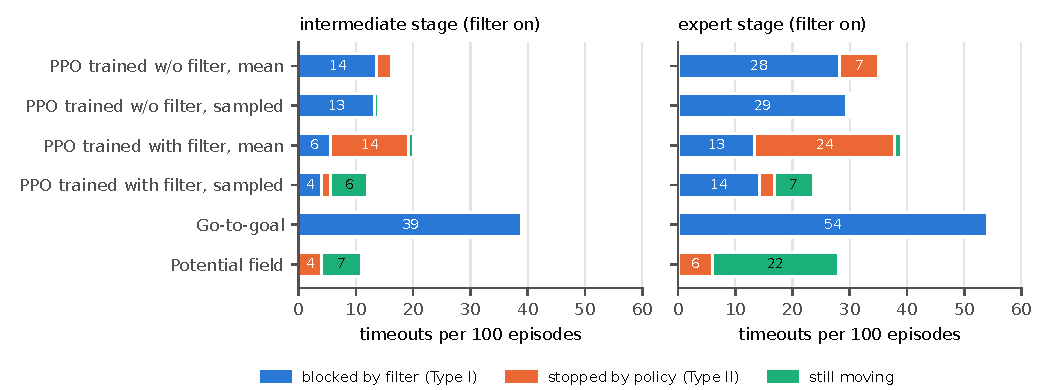
\includegraphics[width=\linewidth]{stall_taxonomy.pdf}
\caption{Timeouts per 100 episodes with the filter on, by stall class (Definition~\ref{def:stall}). PPO: five seeds $\times$ 100 scenarios; baselines: 100 scenarios. Source: \texttt{research/audit\_outputs/stall\_taxonomy\_all.csv}.}
\label{fig:taxonomy}
\end{figure}

\begin{table}[t]
\centering\small
\caption{Timeout classes with the filter on (counts; PPO over 500 episodes per row, baselines over 100). Source: \texttt{research/audit\_outputs/stall\_taxonomy\_all.csv}.}
\label{tab:taxonomy}
\begin{tabular}{@{}lcccccc@{}}
\toprule
 & \multicolumn{3}{c}{Intermediate} & \multicolumn{3}{c}{Expert} \\
\cmidrule(lr){2-4}\cmidrule(l){5-7}
Condition & Type I & Type II & moving & Type I & Type II & moving \\
\midrule
PPO trained w/o filter, mean & 68 & 13 & 0 & 141 & 34 & 0 \\
PPO trained w/o filter, sampled & 66 & 0 & 4 & 147 & 1 & 2 \\
PPO trained with filter, mean & 28 & 68 & 4 & 67 & 122 & 6 \\
PPO trained with filter, sampled & 20 & 8 & 32 & 71 & 13 & 34 \\
Go-to-goal & 39 & 0 & 0 & 54 & 0 & 0 \\
Potential field & 0 & 4 & 7 & 0 & 6 & 22 \\
\bottomrule
\end{tabular}
\end{table}

\subsection{The geometry of filter-blocked stalls matches the analysis}
Proposition~\ref{prop:cone} predicts that a robot blocked at the boundary heads less than $90^\circ$ from the obstacle direction. The data confirm this (Figure~\ref{fig:geometry}a).
\begin{itemize}
  \item 617 of the 618 filter-blocked stalls of all PPO conditions have a heading below $90^\circ$; the remaining one is at $91.3^\circ$. The median is $66.8^\circ$, so the robots are typically not facing the obstacle head-on.
  \item The obstacle barrier at the end of these stalls is at most 4.2\,mm, consistent with the geometric decay in Corollary~\ref{cor:stall}.
  \item In all 618 stalls, the active barrier is an obstacle: no wall barrier is below 1\,mm.
\end{itemize}
Self-stops, in contrast, are spread over barrier values from 0 to 1.4\,m (Figure~\ref{fig:geometry}b). This is consistent with Lemma~\ref{prop:typeII}: at these stops, the speed is set by the policy's command, not by the test-time speed limit. Whether the filter shaped this behaviour during training is discussed in Section~\ref{sec:discussion}.

\begin{figure}[t]
\centering
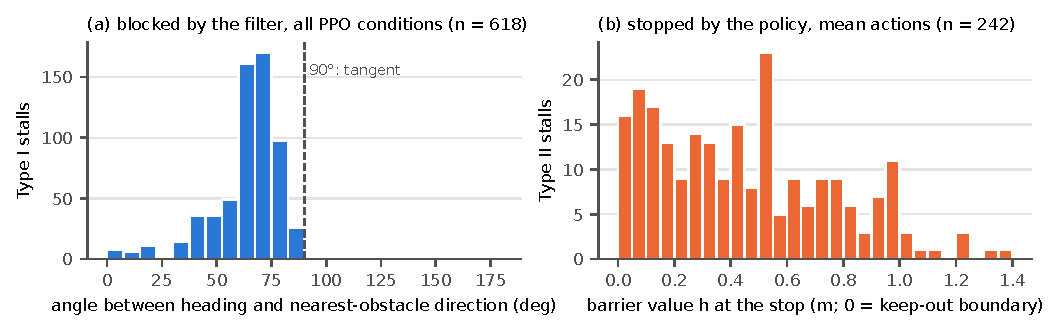
\includegraphics[width=\linewidth]{stall_geometry.pdf}
\caption{(a) Heading relative to the nearest obstacle at the end of filter-blocked stalls (all PPO conditions, both stages); the dashed line marks $90^\circ$ (tangent). (b) Barrier value at self-stops (PPO, mean actions). Source: \texttt{research/audit\_outputs/stall\_taxonomy\_all.csv}.}
\label{fig:geometry}
\end{figure}

\subsection{Training with the filter shifts the mechanism; sampling removes self-stops}
Paired comparisons (Figure~\ref{fig:paired}) quantify both effects.
\begin{itemize}
  \item \textbf{Training with the filter.} On the expert stage, it lowered the filter-blocked rate by 14.8 points [5.6, 24.4] and raised the self-stop rate by 17.6 points [8.2, 27.0]. On the intermediate stage, the corresponding changes were $-8.0$ [$-14.8$, $-1.8$] and $+11.0$ [5.6, 17.2].
  \item \textbf{Sampled actions} (agent trained with the filter). The expert self-stop rate fell by 21.8 points [12.4, 31.6], while the filter-blocked rate did not change ($+0.8$ [$-7.6$, 10.0]).
  \item \textbf{Success.} Sampling raised expert success by 15.4 points [7.8, 24.0] for the filter-trained agent, against 5.0 [0.4, 10.4] for the agent trained without the filter.
\end{itemize}
Stochastic deployment therefore acts on the learned mechanism only. The filter-blocked stalls persist, as Proposition~\ref{prop:cone} suggests they should for any policy that keeps a heading within $90^\circ$ of the obstacle.

\begin{figure}[t]
\centering
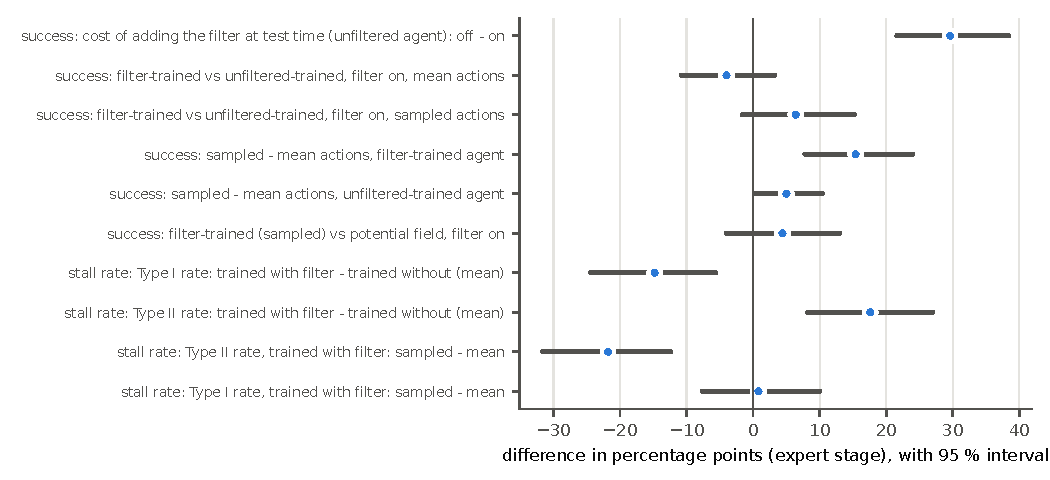
\includegraphics[width=\linewidth]{paired_differences.pdf}
\caption{Paired differences (expert stage) with 95\,\% paired hierarchical bootstrap intervals. Success differences: \texttt{research/audit\_outputs/paired\_comparisons\_expert.csv}; stall-rate differences: \texttt{paper\_draft/generated/stats.json}.}
\label{fig:paired}
\end{figure}

\subsection{Sources of uncertainty}
The decomposition of expert success shows how much the test scenario matters. Depending on the condition, the scenario term accounts for 25--86\,\% of the sum of squares, against under 2\,\% for the seed term. Seed-only intervals such as those in Table~\ref{tab:main} therefore describe reproducibility of training on these 100 scenarios; they understate the uncertainty about the scenario distribution. An approximate fit of interval width to the number of seeds and scenarios suggests that about 10 seeds and 1{,}000 scenarios per stage would give half-widths near 4--5 points for differences of this kind. Beyond about 1{,}000 scenarios, more seeds help more than more scenarios.

\subsection{Replication on previously unused scenarios}
On the 500 fresh expert scenarios (5{,}000 episodes per condition, mean actions), the taxonomy and both training contrasts replicate (Table~\ref{tab:fresh}).
\begin{itemize}
  \item Filter-blocked stalls make up 709 of the 792 timeouts of the agents trained without the filter.
  \item Self-stops make up 577 of the 903 timeouts of the agents trained with it.
  \item Training with the filter lowered the filter-blocked rate by 16.5 points [10.1, 22.8] and raised the self-stop rate by 19.8 points [12.8, 26.1].
\end{itemize}
Both effects are close to those on the original test set. In this larger sample, expert success of the filter-trained agents was also lower than that of the agents trained without the filter, by 4.4 points [0.2, 8.5]. This comparison was exploratory, not one of the pre-registered tests. There were no collisions in the 10{,}000 fresh-scenario episodes, and the minimum clearance was 0.30\,m.

\begin{table}[t]
\centering\small
\caption{Pre-registered evaluation on 500 previously unused expert scenarios (five agents per row, 2{,}500 episodes, mean actions). $\kappa$: heading escape (0 = plain filter). Source: \texttt{research/experiments/lightweight/results/summary.json}.}
\label{tab:fresh}
\begin{tabular}{@{}llccccc@{}}
\toprule
Agents & $\kappa$ & Success (\%) & Timeouts & Type I & Type II & moving \\
\midrule
trained w/o filter & 0 & 68.3 & 792 & 709 & 81 & 2 \\
trained w/o filter & 0.5 & 75.6 & 611 & 523 & 85 & 3 \\
trained with filter & 0 & 63.9 & 903 & 297 & 577 & 29 \\
trained with filter & 0.5 & 64.0 & 901 & 244 & 615 & 42 \\
trained with filter, final checkpoints & 0 & 59.1 & 1023 & 123 & 870 & 30 \\
\bottomrule
\end{tabular}
\end{table}

\subsection{Self-stops are not an artefact of checkpoint selection}
The final checkpoints of the filter-trained runs have more self-stops than the selected checkpoints: $+11.7$ points [3.0, 20.8]. They have fewer filter-blocked stalls ($-7.0$ [$-13.0$, $-1.5$]) and lower success ($-4.8$ [$-8.8$, $-1.2$]). The increase comes from the three seeds whose selected checkpoint was from early in training (0.1--0.3M steps). Self-stops in these seeds rose from 139, 51 and 105 to 205, 174 and 206. In the seed whose best checkpoint is its final one, the results are identical. Longer training with the filter therefore strengthens the self-stopping behaviour rather than removing it.

\subsection{Remedies}
\paragraph{Heading escape (test time, frozen agents).} With $\kappa=0.5$ (Table~\ref{tab:fresh}), the filter-blocked rate of the agents trained without the filter fell by 7.4 points [4.8, 10.2], and their success rose by 7.2 points [5.0, 9.7]. The reduction held in every seed. Self-stops of the filter-trained agents did not change ($+1.5$ [$-0.8$, $3.9$]), nor did their success ($+0.1$ [$-2.2$, $2.4$]). This is expected. The escape is triggered only when the filter reduces the commanded speed, which never happens while the policy commands zero speed (Lemma~\ref{prop:typeII}). A heading change triggered during a stop could in principle change the policy's observation and release it, but we did not test this. There were no collisions, as Lemma~\ref{prop:heading} guarantees. The effect is real but small. It is below the 10-point threshold we fixed in advance, and 523 of the remaining 611 timeouts of these agents are still filter-blocked. A one-step heading rule is therefore not enough to resolve Type~I stalls; it is a lower bound on what filter-level heading changes can do.

\paragraph{Correction penalty.} \evreq{E1a: PPO with the correction-penalty term of~\cite{pizarro2025filtering} ($\alpha=1$, our one-step filter, no safe resets), compared with an identical control. Five seeds and 300k steps per arm. The pre-registered primary contrast uses the policy mean on 500 previously unused expert scenarios (seed base $5\cdot10^6$). The 300 existing test scenarios and sampled actions are secondary. This needs training. A one-seed pilot (150k steps per arm) was run only to check the implementation and the cost. It was evaluated on the fresh scenarios of this section (seed base $9\cdot10^6$), not on the E1a primary set. It showed no large effect and is inconclusive by its pre-registered rule, so it supports no claim here. The multi-seed E1a is still required; see minimum\_experiments.md.}

%=====================================================================
\section{Discussion}\label{sec:discussion}
%=====================================================================
\paragraph{Two different problems.} Most discussions of filter-induced deadlock treat it as one problem of the filter~\cite{reis2021undesired,tan2024undesired}. Our data show two different problems, and which one dominates depends on the training setup. A policy that never saw the filter keeps pushing at the boundary. It is held there because, by Proposition~\ref{prop:cone}, no heading within $90^\circ$ of the obstacle admits motion. This is the learned-policy counterpart of the undesired boundary equilibria of CBF-QPs. A policy trained with the filter is blocked less often, but it mostly stops on its own, typically when an obstacle lies between it and the goal. By Lemma~\ref{prop:typeII}, at the steps where it commands a near-zero speed, no test-time speed limit can make it move. Whether the filter contributed to this behaviour during training is a separate question, discussed next.

\paragraph{Why do filter-trained policies stop?} We separate what is observed from what is hypothesised.
\begin{itemize}
  \item \textbf{Observed.} Self-stops occur at a positive barrier value (median 0.41\,m), mostly when the goal lies roughly in the direction of the nearest obstacle (89 of 122 expert self-stops within $45^\circ$). They are much less frequent in agents trained without the filter: 34 vs.\ 122 of 500 expert episodes on the original scenarios, and 81 vs.\ 577 of 2{,}500 on the fresh scenarios. Sampled actions remove most of them. A heading escape that is triggered by speed reductions leaves them unchanged. They are more frequent at the final training checkpoints than at the selected ones.
  \item \textbf{Not established.} The cause. None of these observations is a causal test, and we have no intervention on the training process that isolates a mechanism.
\end{itemize}
We consider two candidate explanations. The first is \emph{action aliasing} in the filtered environment. Every sampled speed $v\le0$ is executed as $0$, and every speed above the limit is executed as the limit. Within these sets the executed action, and therefore the return, does not depend on the sampled value, so the return carries no information about which of these samples to prefer. Related effects of clipping and projection on policy gradients are documented: variance from ignoring action bounds~\cite{fujita2018capg}, bias of Gaussian policies under bounded actions~\cite{chou2017beta}, zero gradients under projection layers~\cite{lin2021zerogradient}, and the need for corrections when projecting onto a safe set~\cite{gros2020projection}. Our setting is closest to clipping after sampling, as studied by Fujita and Maeda, because the filter acts in the environment and the buffer stores the policy's own sample. Those analyses concern gradient variance and bias, not navigation behaviour, so they make aliasing plausible but do not show that it causes self-stops. Under this explanation, the mean could drift into the stopping region near obstacles, where forward commands were often truncated during training, and sampling would occasionally leave it. Both points are consistent with the observations, but not specific to this explanation. The second explanation is the reward: the non-potential-based risk penalty may make stopping near obstacles attractive. The two explanations are not exclusive.
\begin{hypothesis}
Type~II stops arise mainly from aliasing rather than from the reward. Then a policy whose distribution respects the action bounds (for example a Beta policy~\cite{chou2017beta}), or a clipping-aware gradient estimator~\cite{fujita2018capg}, should reduce them, while removing the risk penalty should not. \evreq{Untested; minimum\_experiments.md, E4.}
\end{hypothesis}

\paragraph{Relation to theory on filtered training.} Oh et al.~\cite{oh2026optimal} prove that RL under a perfect, least-restrictive filter preserves optimality. Such a filter intervenes if and only if the nominal action would make the state leave the maximal controlled-invariant subset of the safety constraint. The filter studied here is not least-restrictive in this sense, under the following assumption and model.
\begin{itemize}
  \item \textbf{Assumption.} The safety constraint is the margin set $\mathcal S$ that our filter enforces.
  \item \textbf{Controlled-invariant set.} In the model \eqref{eq:dyn}, $v=0$ is admissible and keeps the position fixed. Every state whose position lies in $\mathcal S$ can therefore be kept in $\mathcal S$ indefinitely, so the maximal controlled-invariant set consists of all such states. A least-restrictive filter then intervenes only when the next position would leave $\mathcal S$.
  \item \textbf{Exit condition.} The bound used in the proof of Lemma~\ref{lem:inv}, $h_k(p_{t+1})\ge h_k(p_t)-\Delta t\,v_t\,a_k(p_t,\theta_t)$ (with equality for walls), shows that leaving $\mathcal S$ through a closing barrier $k$ ($a_k>0$) in one step requires $v_t\,a_k>h_k/\Delta t$. This is a necessary condition, not a sufficient one. For an oblique approach to an obstacle, the exact speed at which the next position leaves $\mathcal S$ can be larger.
  \item \textbf{Comparison.} Our filter limits the same quantity to $v_t\,a_k\le\gamma h_k$. Both bounds are in m/s, and their ratio is $\gamma\Delta t=0.05$. For a given state, heading and closing barrier, the filter's speed cap $\gamma h_k/a_k$ is therefore at most one twentieth of the speed at which a least-restrictive filter would have to intervene for that barrier. Because the exit condition is necessary and $v\le v_{\max}$, a least-restrictive filter can act on barrier $k$ only where $h_k<a_k v_{\max}\Delta t\le0.1$\,m.
\end{itemize}
If the safety constraint were collision avoidance without the margin, the maximal controlled-invariant set would be larger, and a least-restrictive filter would intervene even less. Oh et al.'s result therefore does not apply directly to our filter, and it does not tell us how much of the gap the filter itself causes. Our reading that much of the remaining gap is a learning problem rests on our own evidence instead:
\begin{itemize}
  \item the oracle finds a margin-keeping path in every test scenario;
  \item most stalls of filter-trained agents are self-stops at a positive barrier value, where the speed is set by the policy's near-zero command rather than by the test-time speed limit (Lemma~\ref{prop:typeII}).
\end{itemize}
This does not exclude that the filter shaped the stopping behaviour during training, which is the aliasing explanation above. Whether a less restrictive filter, for example a larger $\gamma$, would reduce the filter-blocked stalls is open.

\paragraph{Implications for remedy design.} Lemma~\ref{prop:heading} means that heading-level remedies come at no cost to the one-step guarantee. The simple escape tested here helps, but only modestly. A heading rule that looks one step ahead cannot plan a way around an obstacle. Multi-step or planning-level recoveries are the natural next candidates, for example task-aware recovery planning as in~\cite{banerjee2024dmps}. By Lemma~\ref{prop:typeII}, a remedy acting only on the test-time speed limit, such as a less conservative $\gamma$, cannot produce motion at steps where the policy commands a near-zero speed. It could still change earlier parts of the trajectory, which we did not test. A heading escape triggered only by speed reductions did not reduce self-stops in our evaluation. The correction penalty~\cite{pizarro2025filtering} is an established method. In their formulation the certified action respects the input constraints. In our implementation, $u^{\mathrm{exec}}$ is the action after the action bounds and the filter. The term therefore penalises both the filter's truncation and the box clipping of $v\le0$. It may therefore act on both mechanisms. Whether it does so in navigation is the open question that E1 addresses, and this is why it is the most important missing baseline.

%=====================================================================
\section{Limitations and threats to validity}
%=====================================================================
\begin{itemize}
  \item \textbf{External validity.} 2D simulation with exact Euler kinematics, static circular obstacles, exact state for the filter and a known map. Nothing was tested on a robot, and no finite simulation establishes real-world safety. The filter's guarantee holds at the sampled states. Between samples, the chord bound limits the penetration to about 1.4\,mm for the generated obstacle sizes; continuous-time motion is not covered.
  \item \textbf{Scenario design.} Goal clipping shortens many goal distances. Three trivial scenarios add 1--2 points to every success rate in their stages. The layouts are fairly open: the median oracle path is 6--8\,\% longer than the straight line.
  \item \textbf{Test-set reuse.} The margin, the sampled-action evaluation and the stall analysis were all developed on the same test scenarios. The pre-registered evaluation on 500 unused scenarios reduces, but does not remove, this threat. Those scenarios come from the same generator, and only the expert stage, mean actions and one value of $\kappa$ were tested. The sampled-action variant of that evaluation and the final checkpoints of the agents trained without the filter were planned but not run.
  \item \textbf{Statistical power.} Five seeds per variant, with 100 scenarios per stage on the original test set and 500 on the fresh set. The intervals are approximate, and there is no multiplicity correction beyond the pre-registered decision rules.
  \item \textbf{Artefacts.} The final checkpoints used for the checkpoint-selection analysis are not yet in the public repository.
  \item \textbf{Construct validity of the taxonomy.} The class thresholds are heuristic, but varying the displacement threshold, the share threshold and the window length changed the expert counts by at most 4.
  \item \textbf{Baselines and tuning.} PPO hyperparameters were not tuned for the filtered setting, the potential field was tuned by hand, and published safe-RL and classical baselines are missing.
  \item \textbf{Privileged feature.} The proximity feature in the observation is computed from the true map.
\end{itemize}

%=====================================================================
\section{Conclusion}
%=====================================================================
A one-step discrete-time CBF filter makes learned navigation policies collision-free in simulation, but it does not make them live. Two elementary properties of the filter frame the analysis: its one-step guarantee is independent of the turn rate, and the headings admitting motion collapse to a half-plane at the boundary. Empirically, learned policies deadlock behind the filter by two distinct mechanisms. A policy trained without the filter is blocked by the filter at the boundary, while a policy trained with the filter mostly stops itself before it. Stochastic deployment removes the second mechanism but not the first. A test-time heading escape reduces the first modestly and leaves the second untouched. In these runs, longer training with the filter made the second more frequent. The results indicate which part of the problem a filter-level change can address and which part has to be addressed in training. The cause of the self-stops is not yet established. \evreq{Whether the published correction penalty resolves either mechanism (E1) is the main open question.}

\section*{Data and code availability}\label{sec:avail}
Code, committed checkpoints, per-episode results and analysis scripts: \url{https://github.com/pouyapd/SafeNav-RL}. Benchmark: \path{results/benchmark/}; sampled-action evaluation: \path{results/stochastic_eval/}; stall taxonomy: \path{research/scripts/stall_taxonomy.py}; figures and statistics in this paper: \path{research/scripts/paper_figures_stats.py}; pre-registered fresh-scenario evaluation, heading escape and checkpoint comparison: \path{research/experiments/lightweight/} (protocol, runner, analysis and per-episode results). \evreq{Archive a tagged release with a DOI (e.g.\ Zenodo) before submission.}

\bibliographystyle{unsrtnat}
\bibliography{references}
\end{document}
